% adopted from "Riddles in the Dark" template on Overleaf
% incorporated ideas from "Mailmerged Conference Name Cards" template 
\documentclass[grid,avery5371]{flashcards}

% include font icons
\usepackage{fontawesome}

% format url
\usepackage{hyperref}

% specify the variant (AV, AI, LLM, etc) among available card decks.
\newcommand{\deck}{flow}

% read card info from external file
\usepackage{datatool}
%% The "database" is a comma-separated values (CSV) file.
%% The first line should contain the column headers, without space characters, e.g.
%% Name,JobTitle,Department
%%
%% If a field value contains a comma, then the field value needs to be surrounded with double quotes, e.g. 
%% John Smith,Lecturer,"School of Science, Mathematics and Engineering"
%%
%% Spreadsheet applications can usually export such a .csv file.
%%
%% If field values are expected to contain LaTeX special characters like $, &, then use \DTLloadrawdb{data}.csv instead.
\DTLloaddb{prompt}{prompts-\deck.csv}

\DTLloaddb{response}{responses-\deck.csv}

\usepackage[utf8]{inputenc}
\usepackage[T1]{fontenc}
\usepackage{ebgaramond}
\usepackage{tikz}

\usepackage{multicol}

\geometry{headheight=12pt,footskip=4pt}
\usepackage{fancyhdr}
\pagestyle{fancy}
\fancyhf{}
\renewcommand{\headrulewidth}{0pt}
\chead{\small What could go wrong? ({\sc \deck} deck) }

\title{What could go wrong?}
% compiled by:
\author{Matthijs den Besten}
% based on work by Nik Martelaro
% see resitory at https://github.com/mdbesten/what-could-go-wrong-llm
\cardbackstyle[\Huge]{plain}
\cardfrontstyle[\large]{headings}

\begin{document}

\cardfrontfoot{What could go wrong?\qquad\faicon{creative-commons}}

\begin{flashcard}[\faicon{gamepad}\quad Gameplay Instructions]{
%\begin{turn}{180}
%\Rotatebox[origin=c]{90}{%
{\bf\small During the game}
\begin{multicols}{2}
\begin{enumerate}\tiny \setlength{\itemsep}{.5ex}
    \item Take notes on ideas that you have not thought about before
    \item Some of the cards are causes, others are effects. Don’t worry about what the game designers intended with each card, go where the discussion is best.
    \item Some of the cards may be upsetting. (Such as, a person is abused.)
    \item It’s fine to take time to have discussion.
    \item Try not to get sidetracked, though!
\end{enumerate}
\end{multicols}
%}
%\end{turn}{180}
}
{\bf\small What could go wrong?---Gameplay Instructions}
\begin{multicols}{2}
    \begin{enumerate}\tiny \setlength\itemsep{.2ex}
        \item All players draw 5 event cards from their stack.
        \item Use the spinner to select the Card Czar.
        \item The Card Czar reads a black prompt card to the group.
        \item Players think strategically about a card and submit it face down, or a combo in the case of the Wildcard Round, for the best match with the prompt.
        \item \textbf{Wildcard Round: Introduced at a set game point, like after every third round. Players can use two white cards for a chance at double points if both cards of one player are chosen by the Card Czar.}
        \item The Card Czar reveals and chooses the most fitting or humorous cards. Chosen cards' user earn points: +1 normally, \textbf{+2 during the Wildcard Round if both cards of one player are chosen}.
        \item Discuss the chosen cards and award +1 point for compelling contributions.
        \item After discussing, the next player becomes the Card Czar. Each player then draws new cards, so that they again have 5 cards in their hand.
    \end{enumerate}
\end{multicols}
\end{flashcard}



% Adopted from http://www.unm.edu/~unmvclib/gamification/assessment/gameevaluationcriteria.pdf
\begin{flashcard}[\faicon{meh-o}\quad Game Evaluation Criteria]{
    \begin{itemize}\tiny \setlength{\itemsep}{.1ex}
        \item Category Biases
        \item Scale 1 to 7
        \begin{multicols}{3}
        \begin{itemize}
            \item Clarity
            \item Flow
            \item Balance
            \item Length
            \item Integrity
            \item Fun
        \end{itemize}
        \end{multicols}
        \begin{multicols}{2}
        \item Strongest Point
        \item Weakest Point
        \item One Change
        \item Comparable Games
        \end{multicols}
    \end{itemize}
    }
    {\bf\small What could go wrong?---Game Evaluation}
    \small
    \begin{tabular}{l|c|c|c|c|}
        & 1 & 3 & 5 & 7\\
    \hline
    {\em Clarity} & Opaque & Muddy & Transparent & Water-clear \\
    {\em Flow} & Cumbrous & Fraught & Smooth & Natural \\
    {\em Balance} & Broken & Fluky & Sensible & Fair\\
    {\em Length} & Wrong & Unfit & Apt & Perfect \\
    {\em Integrity} & Eristic & Erratic & Coherent & Sound \\
    {\em Fun} & Offputting & Boring & Engaging & Exciting \\
    \hline
    \end{tabular}
\end{flashcard}



\begin{flashcard}[\faicon{star}\quad Wildcard Round]{
\begin{center}

\begin{tikzpicture}[scale=1]    
    % Title with customized font
    \node[align=center, font=\bfseries\Large] at (4cm, 4.5cm) {Wildcard};
    
    % Additional customization
    % You can add more elements here to customize the first side further
    
\end{tikzpicture}
\end{center}
}
{\bf\small Wildcard Round}
\begin{center}
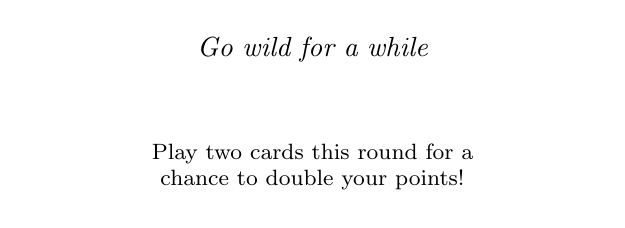
\begin{tikzpicture}[scale=1]
    % Card background    
    
    % Quote
    \node[align=center, font=\itshape, text width=6cm] at (4cm, 2.5cm) {Go wild for a while}; % Adjusted position and width
    
    % Instruction Text
    \node[text width=7cm, align=center, font=\footnotesize] at (4cm,1cm) {Play two cards this round for a chance to double your points!}; % Adjusted position and width
    

\end{tikzpicture}
\end{center}
\end{flashcard}




\DTLforeach{prompt}{%
    %% Map each column header in your .csv file to a command
	\Description=PROMPT,%
    \Category=LABEL,%
    \Id=NUMBERS%
}{%%%  Start designing your output text!
\begin{flashcard}[\deck:\quad\Id\quad\DTLifnull{\Category}{}{\Category}]{%
%\begin{verse}[\versewidth]
\Description
%\end{verse}
}
\faicon{tasks}\quad{\sc \deck}\\
\end{flashcard}
}

\DTLforeach{response}{%
    %% Map each column header in your .csv file to a command
	\Description=RESPONSE,%
    \Category=LABEL,%
    \Id=NUMBERS%
}{%%%  Start designing your output text!
\begin{flashcard}[\deck:\quad\Id\quad\DTLifnull{\Category}{}{\Category}]{%
\Description
}
\faicon{reply}\quad{\sc \deck}\\
\end{flashcard}
}

\end{document}
